\documentclass{article}\usepackage[]{graphicx}\usepackage[]{xcolor}
% maxwidth is the original width if it is less than linewidth
% otherwise use linewidth (to make sure the graphics do not exceed the margin)
\makeatletter
\def\maxwidth{ %
  \ifdim\Gin@nat@width>\linewidth
    \linewidth
  \else
    \Gin@nat@width
  \fi
}
\makeatother

\definecolor{fgcolor}{rgb}{0.345, 0.345, 0.345}
\newcommand{\hlnum}[1]{\textcolor[rgb]{0.686,0.059,0.569}{#1}}%
\newcommand{\hlstr}[1]{\textcolor[rgb]{0.192,0.494,0.8}{#1}}%
\newcommand{\hlcom}[1]{\textcolor[rgb]{0.678,0.584,0.686}{\textit{#1}}}%
\newcommand{\hlopt}[1]{\textcolor[rgb]{0,0,0}{#1}}%
\newcommand{\hlstd}[1]{\textcolor[rgb]{0.345,0.345,0.345}{#1}}%
\newcommand{\hlkwa}[1]{\textcolor[rgb]{0.161,0.373,0.58}{\textbf{#1}}}%
\newcommand{\hlkwb}[1]{\textcolor[rgb]{0.69,0.353,0.396}{#1}}%
\newcommand{\hlkwc}[1]{\textcolor[rgb]{0.333,0.667,0.333}{#1}}%
\newcommand{\hlkwd}[1]{\textcolor[rgb]{0.737,0.353,0.396}{\textbf{#1}}}%
\let\hlipl\hlkwb

\usepackage{framed}
\makeatletter
\newenvironment{kframe}{%
 \def\at@end@of@kframe{}%
 \ifinner\ifhmode%
  \def\at@end@of@kframe{\end{minipage}}%
  \begin{minipage}{\columnwidth}%
 \fi\fi%
 \def\FrameCommand##1{\hskip\@totalleftmargin \hskip-\fboxsep
 \colorbox{shadecolor}{##1}\hskip-\fboxsep
     % There is no \\@totalrightmargin, so:
     \hskip-\linewidth \hskip-\@totalleftmargin \hskip\columnwidth}%
 \MakeFramed {\advance\hsize-\width
   \@totalleftmargin\z@ \linewidth\hsize
   \@setminipage}}%
 {\par\unskip\endMakeFramed%
 \at@end@of@kframe}
\makeatother

\definecolor{shadecolor}{rgb}{.97, .97, .97}
\definecolor{messagecolor}{rgb}{0, 0, 0}
\definecolor{warningcolor}{rgb}{1, 0, 1}
\definecolor{errorcolor}{rgb}{1, 0, 0}
\newenvironment{knitrout}{}{} % an empty environment to be redefined in TeX

\usepackage{alltt}
\title{\textbf{Discussion Assignment 2}}
\author{\textbf{Katherine Wolf}\\ Introduction to Causal Inference (PH252D)\\ \today}
\date{}

% list of latex packages you'll need
\usepackage{float}  % for tables
\usepackage{mathtools}  % for mathematical symbols
\usepackage{bm}  % to bold mathematical symbols like betas
\usepackage{scrextend}  % to indent subsections
\usepackage{xltxtra}
\usepackage{fontspec}
\usepackage{xunicode}
\usepackage[skip=0.5\baselineskip]{caption}  % control caption printing space
\usepackage{longtable}
\usepackage{amsmath}
\usepackage{amsfonts}
\usepackage{bm}
\usepackage{caption}
\usepackage[shortlabels]{enumitem}
\usepackage{txfonts}
\usepackage{dejavu}

% set fonts
\setmainfont{Georgia}
\setsansfont[Scale=MatchLowercase]{Arial}  % sets the sans font
\setmonofont[Scale=MatchLowercase]{DejaVuSansMono}  % sets the monospace font

% make special code formatting
\NewDocumentCommand{\codeword}{v}{%
  \texttt{{#1}}%
}

% set the margins of the document
\usepackage[top=1in, bottom=1in, left=.5in, right=.5in]{geometry}
\setlength\parindent{0pt}



% end the preamble and begin the document
\IfFileExists{upquote.sty}{\usepackage{upquote}}{}
\begin{document}

\maketitle

\section{Instructions}

\section{Background}

\section{Questions to be answered}

\setlength{\leftskip}{0.8cm}

\begin{enumerate}[label=\textbf{\arabic*.}]

  \item \textbf{Specify your observed data.}
  
  \begin{enumerate}[label=\textbf{(\alph*)}]
  
    \item \textbf{What notation do we use to refer to the distribution of the observed data?}
    
    $\mathbb{P}_{\bm{O}}$, as in $\bm{O} = (\bm{W}, \bm{A}, \bm{X}) \sim \mathbb{P}_{\bm{O}}.$
  
    \item \textbf{Specify the link between the SCM and the observed data.}
    
We link the the observed data to the SCM by assuming that we obtained them from a data-generating system described by our SCM, i.e., that each observation in the data represents a draw from the unknown probability distribution $\mathbb{P}_{\bm{U}}$ of the exogenous variables $\bm{U}$, i.e., we drew $\bm{U} = \bm{u}$, that we then plugged into our structural equations $\mathcal{F}$ to output a specific $\bm{X} = \bm{x}$, of which we observed the subset $\bm{O} = \bm{o}$.
    
Thus we assume that the the structural equations $\mathcal{F}$ as applied to $\bm{U} \sim \mathbb{P}_{\bm{U}}$ will identify the distribution $\bm{X} \sim \mathbb{P}_{\bm{X}}$ and, since $\bm{O} \subseteq \bm{X}$, the distribution of its observed subset $\bm{O} \sim \mathbb{P}_{\bm{O}}$. (Since here we assume that $\bm{X} = \bm{O}$, we can write $P_O(O = o) = \sum\limits_{u}P_f(X=x|U=u)P(U=u)) = \sum\limits_{u}I(X(u)=x|U=u)P(U=u)$.)
    
    \item \textbf{What is the statistical model $\mathcal{M}$?}
    
The statistical model $\mathcal{M}$ consists of 

\begin{itemize}

  \item The endogenous variables $\bm{X} = (W, A, Y)$;
  \item The exogenous variables $\bm{U} = (U_W, U_A, U_Y) \sim \mathbb{P}_U$; and
  \item The structural equations $\mathcal{F}$:

\begin{align*}
W &= f_W(U_W) \\
A &= f_A(W,U_A) \\
Y &= f_Y(W,A,U_Y).
\end{align*}

\end{itemize}

The structural equations in directed acyclic graph (DAG) format:
    
\begin{knitrout}
\definecolor{shadecolor}{rgb}{0.969, 0.969, 0.969}\color{fgcolor}
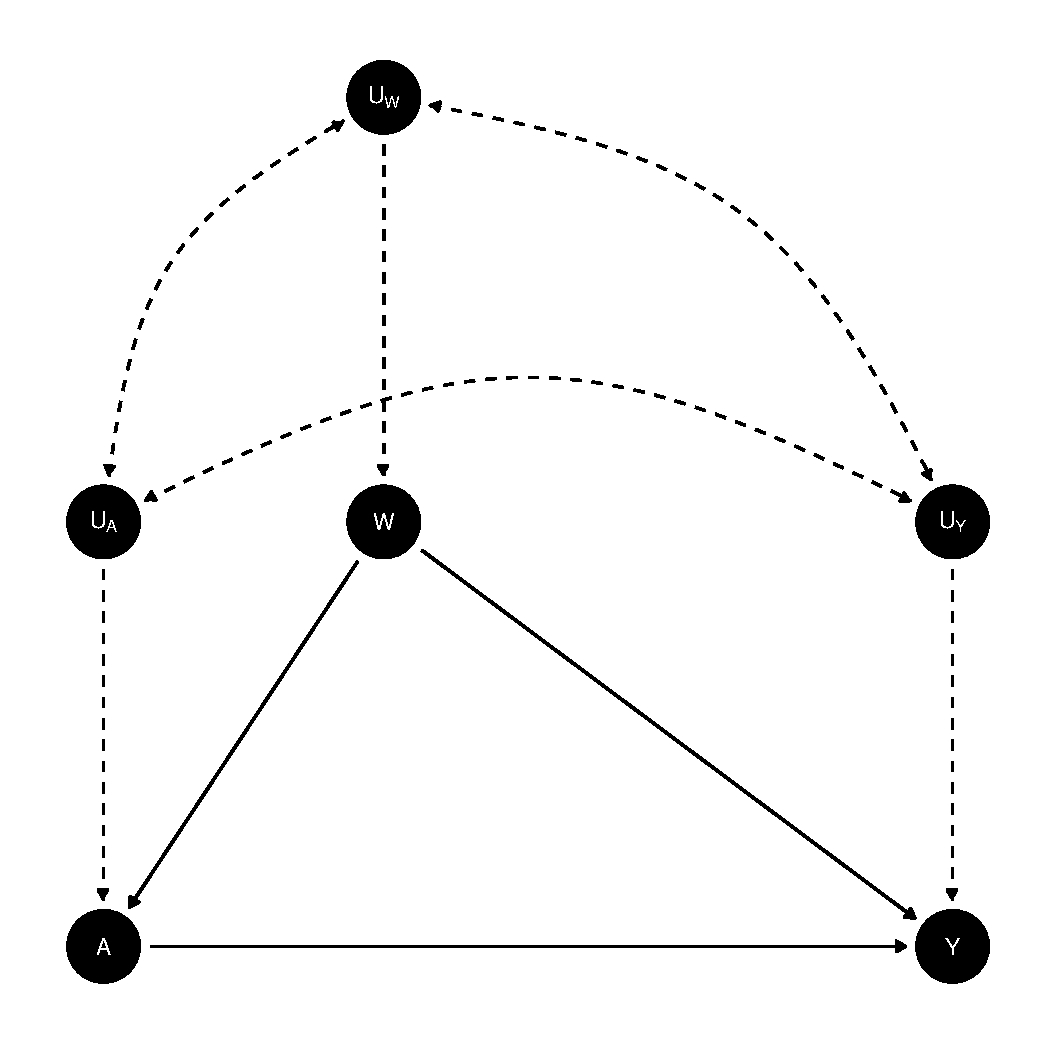
\includegraphics[width=4in]{figure/unnamed-chunk-2-1} 

\end{knitrout}

\textbf{Does the SCM place any restrictions on $\mathcal{M}$?}

There are no independence assumptions, i.e., no restrictions on the distribution of the exogenous variables $\mathbb{P}_{\bm{U}}$. Nor are there any exclusion restrictions aside from the ordering of the recursive, time-ordered SCM.

  \end{enumerate}
    
  \item \textbf{Using the backdoor criterion, assess identifiability of} $\Psi^F(P_{\bm{U},\bm{X}})$.
  
The back-door criterion states that a set of variables $\bm{Z}$ satisfies it with respect to the variable for the exposure of interest $A$ and the variable for the outcome of interest $Y$ if $\bm{Z}$ blocks all unblocked back-door (i.e., with an arrow going into $A$) paths from $A$ to $Y$ without creating any new non-causal associations between $A$ and $Y$.

Another way to state it is that $\bm{Z}$ satisfies the back-door criterion with respect to $(A,Y)$ if
  
  \begin{itemize}
    \item $\bm{Z}$ blocks all paths from $A$ to $Y$ with an arrow into $A$, and
    \item No node in $\bm{Z}$ is a descendant of $A$.
  \end{itemize}
  
If such a set $\bm{Z}$ exists, then the back-door criterion holds, and thus we can identify the effect of $A$ on $Y$, specifically the target causal parameter $\Psi^F(P_{\bm{U},\bm{X}})$, as a parameter of the observed data distribution $\Psi(\mathbb{P}_O)$ by the G-computation formula.
  
Unfortunately, in the SCM $\mathcal{M}^{F}$, $\Psi^F(P_{\bm{U},\bm{X}})$ is not identified, as the only measured variable available for satisfaction of the back-door criterion is $\bm{W}$ (or the empty set), and neither $\bm{W}$ nor the empty set meets the back-door criterion due to the remaining open back-door path between $A$ and $Y$ through $U_A$ and $U_Y$ (including the one through $U_A$, $U_W$, and $U_Y$.)
  
  \begin{enumerate}[label=\textbf{(\alph*)}]
  
    \item \textbf{If not identified, under what assumptions would it be? Are some of these sets of additional assumptions more plausible than others? Are there additional measurements you could make so that the needed identifiability assumptions are more plausible?}
    
    The following DAGs show the three possible working structural causal models that identify $\Psi^F(P_{\bm{U},\bm{X}})$.
    
\begin{itemize}

  \item $\mathcal{M}^{F^*}_1$ assumptions: 
  
  \begin{itemize} 
  
    \item $U_A$ is indepdendent of $U_Y$, i.e., the unmeasured factors $U_A$ that influence energy expenditure $A$ do not affect and are not affected by the unmeasured factors $U_Y$ influencing survival $Y$
    
    \item $U_A$ is indepdendent of $U_W$, i.e., the unmeasured factors $U_A$ that influence energy expenditure $A$ do not affect and are not affected by the unmeasured factors $U_W$ influencing the covariates like smoking, comorbidities, and body fat $W$
    
  \end{itemize}
    
\begin{knitrout}
\definecolor{shadecolor}{rgb}{0.969, 0.969, 0.969}\color{fgcolor}
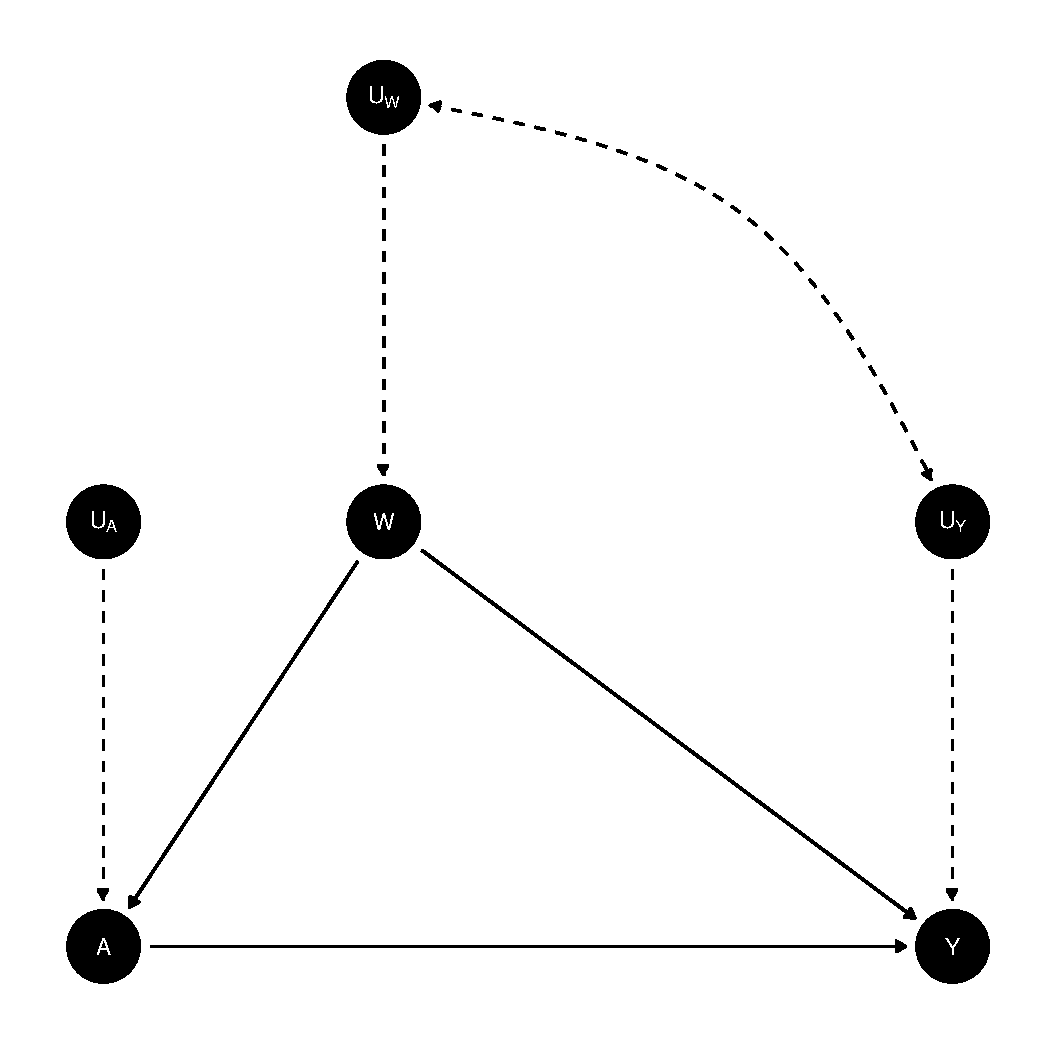
\includegraphics[width=4in]{figure/unnamed-chunk-3-1} 

\end{knitrout}



    
\begin{knitrout}
\definecolor{shadecolor}{rgb}{0.969, 0.969, 0.969}\color{fgcolor}
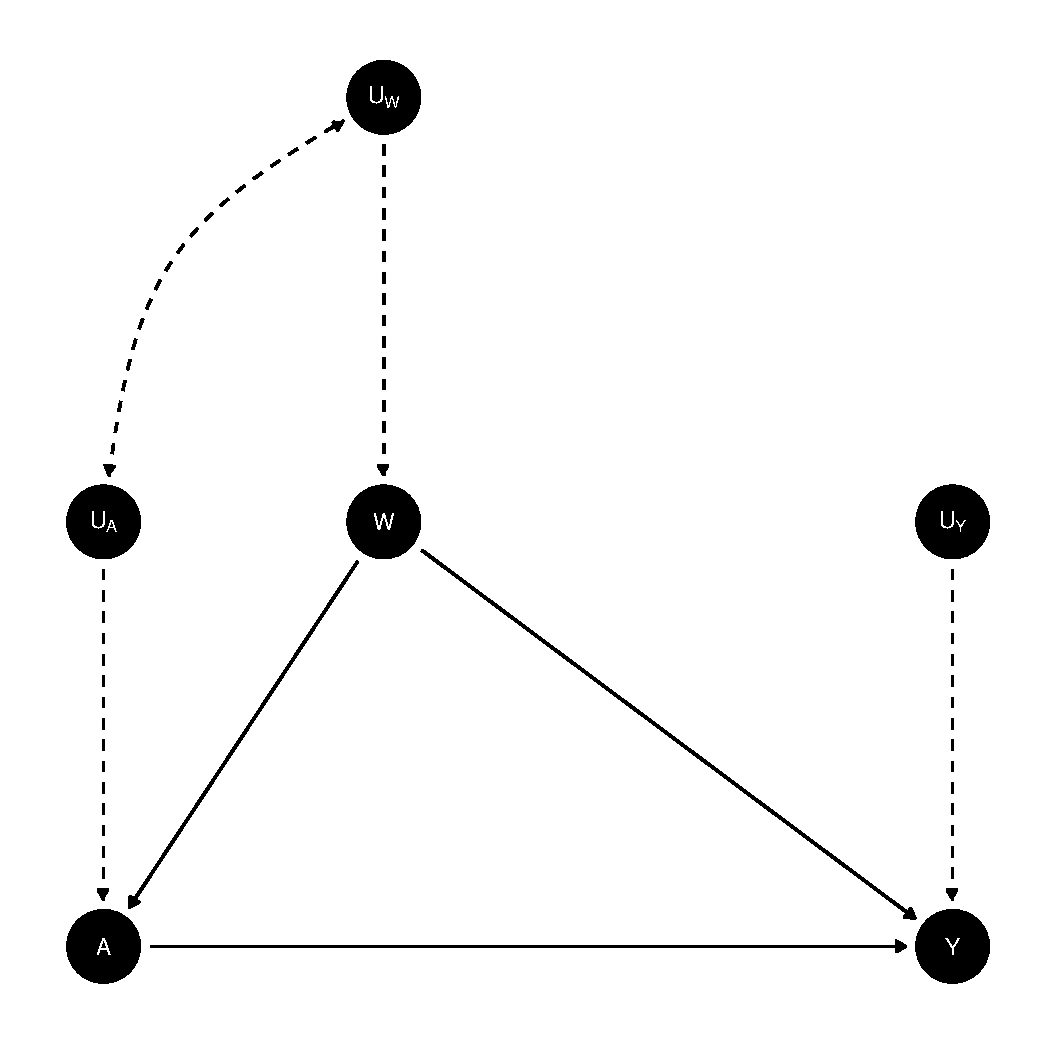
\includegraphics[width=4in]{figure/unnamed-chunk-4-1} 

\end{knitrout}

    
    
    
    
    
   
\begin{knitrout}
\definecolor{shadecolor}{rgb}{0.969, 0.969, 0.969}\color{fgcolor}
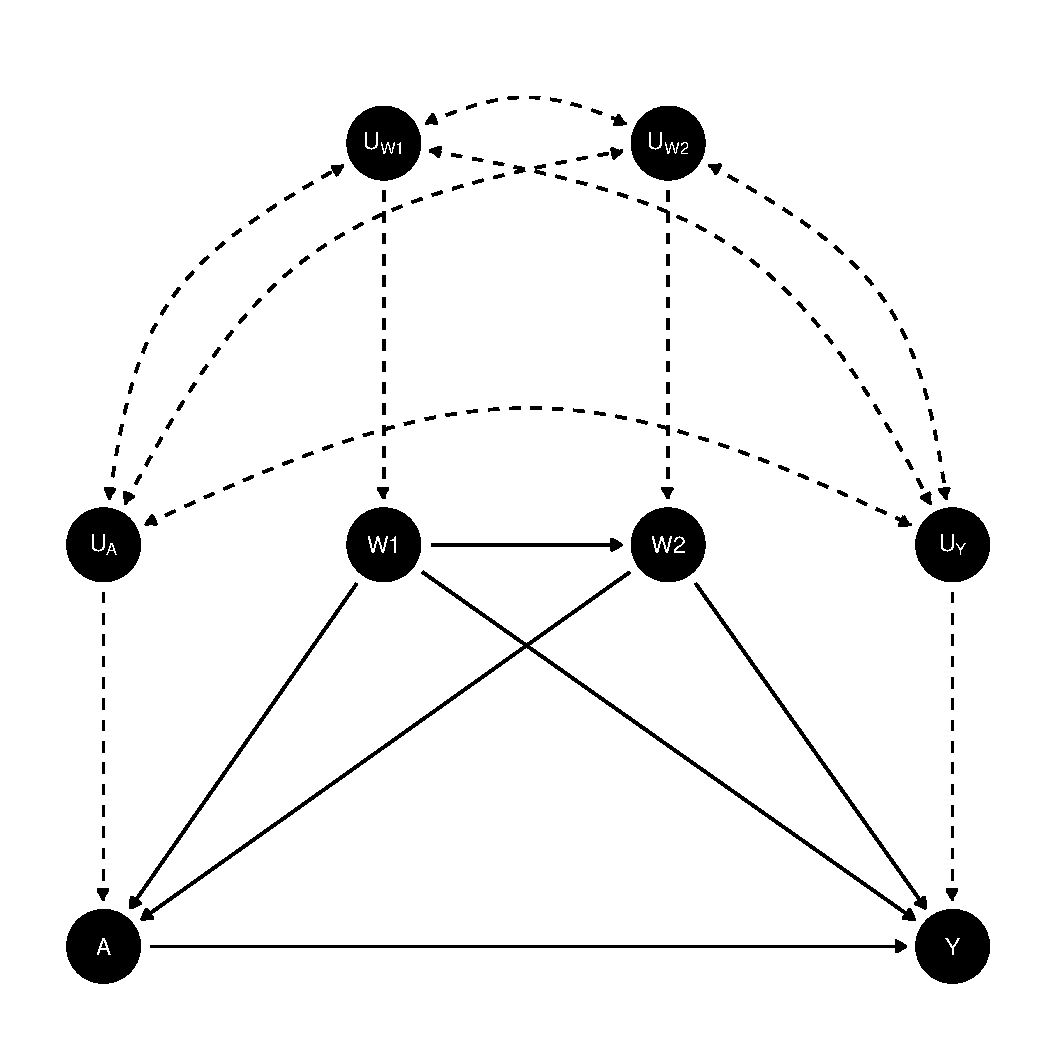
\includegraphics[width=4in]{figure/unnamed-chunk-5-1} 

\end{knitrout}

    
\end{itemize}
 
 
 
 
 
    
    
    \item \textbf{What notation do we use to denote the original SCM, augmented with additional assumptions needed for identifiability?}
    
    $\mathcal{M}^{F^*}$
    
  \end{enumerate}
  
  \item \textbf{Specify the target parameter of the observed data distribution (i.e., the statistical estimand).}
  
  \item \textbf{What is the relevant positivity assumption? Are you concerned about violations of the positivity assumption in your study?}
  
  The relevant positivity assumption is
  
\end{enumerate}

\setlength{\leftskip}{0cm}

\section{Study-specific questions}

\setlength{\leftskip}{0.8cm}

\textbf{The investigators assume no unmeasured common causes of (W, A, Y). Is this necessary? Is this sufficient?} 

\setlength{\leftskip}{0cm}
      
  \end{document} 
